% The 3 x 3 x 5 pre-registered design: arms x task families x metrics = 45 cells.
\documentclass[border=10pt]{standalone}
\usepackage{tikz}
\usepackage{xcolor}
\definecolor{armc}{HTML}{0D9488}
\definecolor{famc}{HTML}{4F46E5}
\definecolor{metc}{HTML}{D97706}
\begin{document}
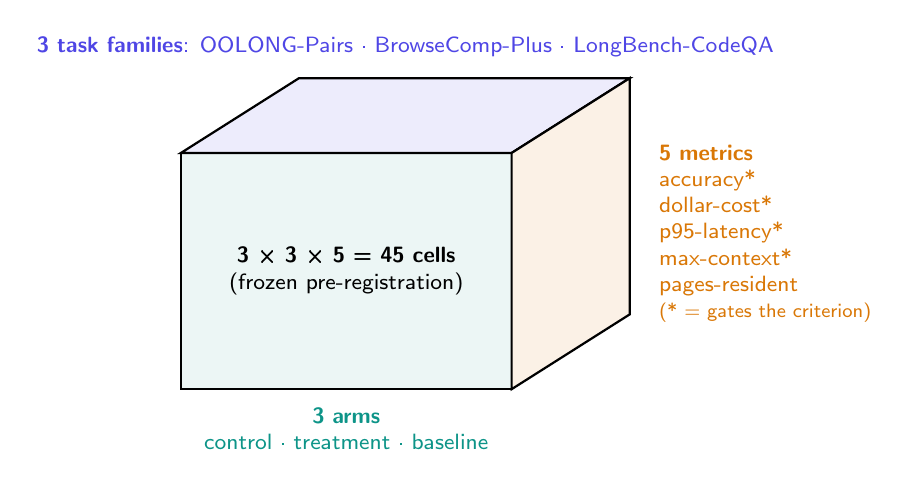
\begin{tikzpicture}[font=\sffamily\footnotesize]
  \def\ax{4.2}\def\ay{3.0}\def\dx{1.5}\def\dy{0.95}
  % front face (arms x metrics)
  \fill[armc!8] (0,0) rectangle (\ax,\ay);
  \draw[thick] (0,0) rectangle (\ax,\ay);
  % top face (depth = families)
  \fill[famc!10] (0,\ay) -- (\dx,\ay+\dy) -- (\ax+\dx,\ay+\dy) -- (\ax,\ay) -- cycle;
  \draw[thick] (0,\ay) -- (\dx,\ay+\dy) -- (\ax+\dx,\ay+\dy) -- (\ax,\ay) -- cycle;
  % right face
  \fill[metc!10] (\ax,0) -- (\ax+\dx,\dy) -- (\ax+\dx,\ay+\dy) -- (\ax,\ay) -- cycle;
  \draw[thick] (\ax,0) -- (\ax+\dx,\dy) -- (\ax+\dx,\ay+\dy) -- (\ax,\ay) -- cycle;

  \node[align=center] at (\ax/2,\ay/2) {\textbf{3 × 3 × 5 = 45 cells}\\(frozen pre-registration)};

  % axis labels
  \node[armc, align=center] at (\ax/2,-0.5) {\textbf{3 arms}\\control · treatment · baseline};
  \node[famc, align=center, anchor=south] at (\ax/2+\dx/2,\ay+\dy+0.15)
    {\textbf{3 task families}: OOLONG-Pairs · BrowseComp-Plus · LongBench-CodeQA};
  \node[metc, align=left, anchor=west] at (\ax+\dx+0.25,\ay/2+\dy/2)
    {\textbf{5 metrics}\\accuracy*\\dollar-cost*\\p95-latency*\\max-context*\\pages-resident\\\scriptsize(* = gates the criterion)};
\end{tikzpicture}
\end{document}
